% Author: Theseas Maroulis
\documentclass[a4paper]{article}
\usepackage{xltxtra}
\usepackage[utf8]{inputenc}
\usepackage[greek]{babel}
\usepackage[a4paper, top=1.5cm, bottom=1.5cm, left=1.5cm,  right=1.5cm]{geometry}
\usepackage{amsmath, amssymb}
\usepackage{graphicx}
\usepackage{fancyhdr}
\usepackage{lastpage}
\usepackage{color}
\usepackage{tabularx}
\usepackage[usenames,table]{xcolor}
\usepackage{enumitem}
\usepackage{booktabs}
\usepackage{tikz}
\usepackage{multirow}
\usepackage[pdfauthor={Θησέας Μαρούλης (std101957@ac.eap.gr)}, pdftitle={Πλη11 Σημειώσεις}, colorlinks=true, linkcolor=blue]{hyperref}
\usepackage{listingsutf8}

\pagestyle{fancy}
\setmainfont[Mapping=tex-text]{DejaVu Sans}
\everymath{\displaystyle}
\renewcommand{\textdexiakeraia}{}

\begin{document}
% \chead{\large \color[HTML]{000090}\bfseries ΕΛΛΗΝΙΚΟ ΑΝΟΙΚΤΟ ΠΑΝΕΠΙΣΤΗΜΙΟ}
% \lfoot{\small{ΓΕ\_4 ΠΛΗ11-ΑΘΗΝΑ\_04 2015-2016}}
\title{Σημειώσεις πλη11}
\author{Θησέας Μαρούλης}
\date{\today}
\lhead{Σημειώσεις πλη11 - Θησέας Μαρούλης}
\lfoot{\small{Θησέας Μαρούλης}}
\cfoot{}
\rfoot{\small{\thepage/\pageref{LastPage}}}


\lstset{
	tabsize=4,
	language={C++},
	frame=single,
	keepspaces=true,
	%nunmbers=left,
	numbersep=5pt,
	breaklines=true,
	commentstyle=\color{gray},
	keywordstyle=\bfseries\color{blue}
}
\maketitle

\pagebreak
\tableofcontents

\section{Μοντέλα Κύκλου Ζωής Λογισμικού}

\subsection{Μοντέλο Καταρράκτη}

\begin{figure}[H]
	\centering
	\includegraphics[width=0.6\textwidth]{waterfall.png}
	\caption{Waterfall model}
\end{figure}


\begin{itemize}
	\item	Καλό για μικρού ή μεσαίου μεγέθους εφαρμογές με απαιτήσεις
		εκ των προτέρων γνωστές.
	\item	Πρόβλημα αν αλλάξουν οι απαιτήσεις κατα την κατασκευή.
	\item	Διάδοση μεγάλη με τάσεις μείωσης.
\end{itemize}


\subsection{Μεντέλο Πρωτοτυποποίησης}

\begin{figure}[H]
	\centering
	\includegraphics[width=0.6\textwidth]{prototyping.png}
	\caption{Prototyping Model}
\end{figure}

\begin{itemize}
	\item	επαναληπτικό μοντέλο που σε κάθε κύκλο κατασκευάζενται
		διαδοχικά πρότυπα με ολοένα περισσότερα χαρακτηριστικά αυτό να γίνει 
		αποδεκτό από τον πελάτη. Κάθε πρότυπο είναι ένα μικρό έργο λογισμικού 
		και μπορεί να χρησιμοποιεί άλλα μοντέλα.
	\item	ιδανικό για μικρές ή μεσαίες εφαρμογές που οι απαιτήσεις τους δεν είναι από την 
		αρχή γνωστές.
	\item	ιδιαίτερη σημασία αποκτά η διοίκηση του έργου.
	\item	διάδοση μικρή με τάσεις αύξησης
\end{itemize}

\subsection{Μοντέλο Λειτουργικής Επαύξησης}

\begin{figure}[H]
	\centering
	\includegraphics[width=0.6\textwidth]{incremental.png}
	\caption{Incremental Model}
\end{figure}

\begin{itemize}
	\item	Κατάτμηση του λογισμικού, εφαρμογή του μοντέλου του καταράκτη σε κάθε τμήμα και
		συνένωση του στο τέλος.
	\item	πλεονεκτήματα είναι η δυνατότητα παράλληλης ανάπτυξης, η οποία τελικά καταλάμβάνει
		μικρότερο χρόνο, καθώς και ο διαδοχικός εμπλουτισμός των λειτουργικών χαρακτηριστικών του.
	\item	μειονέκτημα: ιδιαίτερη βαρύτητα έχει η αρχική κατάτμηση του λογισμικού.
	\item	μειονέκτημα: Οι μεταβολές στις απαιτήσεις μπορεί να κλονίσουν την ανάπτυξη των υπόλοιπων τμημάτων.
	\item	Μεσαίος ως μεγάλο μέγεθος έργου με σαφείς απαιτήσεις από την αρχή.
	\item	διάδοση μικρή με τάση μείωσης.
\end{itemize}

\subsection{Σπειροειδές Μοντέλο}

\begin{figure}[H]
	\centering
	\includegraphics[width=0.6\textwidth]{spiral.png}
	\caption{Spiral Model}
\end{figure}

\begin{itemize}
	\item	Κύκλοι εργασιών με σταδιακή επέκταση των λειτουργικών χαρακτηριστικών της εφαρμογής.
	\item	Εκτίμηση ρίσκου σε κάθε κύκλο.
	\item	Μέγεθος εφαρμογής μεσαίο έως μεγάλο
	\item	Δεκτές οι μεταβολές στις απαιτήσεις
	\item	Αρκετή προσαρμοστικότητα στον κατασκευαστή.
	\item	Διάδοση μικρή με τάσεις μείωσης.
\end{itemize}

\subsection{Μοντέλο Πίδακα}

\begin{figure}[H]
	\centering
	\includegraphics[width=0.6\textwidth]{object_oriented.png}
	\caption{Object Oriented Model}
\end{figure}

\begin{itemize}
	\item	Ανάπτυξη με αντικειμενοστρεφή φιλοσοφία και επαναχρησιμοποίηση έτοιμων συστατικών.
	\item	Κατάλληλο για οποιοδήποτε μέγεθος έργου.
	\item	Δεκτές οι μεταβολές στις απαιτήσεις.
	\item	Αρκετή προσαρμοστικότητα στον κατασκευαστή.
	\item	Διάδοση μικρή.
\end{itemize}

\subsection{Γενικό Μοντελό}

\begin{figure}[H]
	\centering
	\includegraphics[width=0.6\textwidth]{general.png}
	\caption{General Model}
\end{figure}

\begin{itemize}
	\item	Ανάπτυξη σε κύκλους σύμφωνα με τα χαρακτηριστικά και τις δυνατότητες του κατασκευαστή.
	\item	Γενικευμένη μορφή των προηγούμενων μοντέλων κύκλου ζωής.
	\item	Δεκτές οι μεταβολές στις απαιτήσεις.
	\item	Κατάλληλο για οποιοδήποτε μέγεθος έργου.
	\item	Μεγάλη προσαρμοστικότητα στον κατασκευαστή.
	\item	Διάδοση μικρή με ισχυρές τάσεις αύξησης.
\end{itemize}


\section{Απαιτήσεις από το Λογισμικό}

\begin{itemize}
	\item	Λειτουργικές απαιτήσεις
	\item	Μη λειτουργικές απαιτήσεις
		\begin{itemize}
			\item	Απαιτήσεις χρήσης
			\item	Απαιτήσεις αξιοπιστίας
			\item	Απαιτήσεις επιδόσεων
			\item	Απαιτήσεις υποστήριξης
			\item	Απαιτήσεις σχεδίασης
			\item	Απαιτήσεις υλοποίησης
			\item	Απαιτήσεις επικοινωνίας με άλλα συστήματα
			\item	Απαιτήσεις βάσης δεδομένων
			\item	Φυσικές απαιτήσεις
		\end{itemize}
\end{itemize}

\pagebreak
\section{Διάγραμμα Ροής Δεδομένων}

\paragraph{Πηγή ή Αποδέκτης Δεδομένων}
Τα δεδομένα πρέπει πάντοτε να προέρχονται από κάπου και πρέπει να αποστέλλονται σε κάποιον.

\paragraph{Μετασχηματισμός Δεδομένων (αλλάζει την είσοδο σε έξοδο)}
Τα δεδομένα πρέπει πάντοτε να υπόκεινται σε επεξεργασία με
κάποιο τρόπο για να επιτευχθεί η λειτουργία του συστήματος.

\paragraph{Αποθήκη Δεδομένων}
Ο αριθμός των δεδομένων που γράφονται και διαβάζονται πρέπει να είναι ίδιος
στο συνολικό ΔΡΔ.

\begin{itemize}
	\item	Οι ροές εισόδου/εξόδου πρέπει προσεκτικά να καταγράφονται.
	\item	Στο επίπεδο 0 πάντοτε φαίνονται οι εξωτερικές οντότητες (πηγές / αποδέκτες).
	\item	Δώστε ετικέτα σε καθετί.
	\item	Οι εξωτερικές οντότητες μπορεί να επαναλαμβάνονται στο ίδιο διάγραμμα.
	\item	Οι εξωτερικές οντότητες  πρέπει να επαναλαμβάνονται σε όλα τα επίπεδα του ΔΡΔ,
		τουλάχιστον από μία φορά λόγω συνέπειας μεταξύ επιπέδων.
	\item	Κάθε φορά αναλύουμε ένα κύκλο (λειτουργία).
	\item	Η ανάλυση συνεχίζεται μέχρι κάθε κύκλος να αναπαριστά μια απλή και μοναδική λειτουργία 
		που συνδέεται με μια μόνο μονάδα προγράμματος.
	\item	Κάθε ροή δεδομένων (βέλος) μπορεί να αναλύεται στο επόμενο επίπεδο 
		(κάθε ροή δεδομένων καταγράφεται στο λεξικό δεδομένων).
	\item	Δεν περιγράφουμε διαδικαστική λογική (αλγόριθμο).
\end{itemize}

\begin{tabularx}{0.9\textwidth}{|X|X|X|X|}
	\hline
	{} & {Πηγή ή Αποδέκτης} & {Μετασχηματισμός} & {Αποθήκη Δεδομένων} \\
	\hline
	{Πηγή ή Αποδέκτης} & {X} & {\checkmark} & {X} \\
	\hline
	{Μετασχηματισμός} & {\checkmark} & {\checkmark} & {\checkmark} \\
	\hline
	{Αποθήκη Δεδομένων} & {X} & {\checkmark} & {X} \\
	\hline
\end{tabularx}

\begin{figure}[H]
	\centering
	\includegraphics[width=0.9\textwidth]{drd.png}
	\caption{Συμβολισμοί \& Συμβάσεις ΔΡΔ}
\end{figure}


\section{Διάγραμμα Μετάβασης Καταστάσεων}

\begin{figure}[H]
	\centering
	\includegraphics[width=0.5\textwidth]{dmk.png}
	\caption{Συμβολισμοί ΔΜΚ}
\end{figure}

\begin{enumerate}
	\item	Αναγνώριση της οντότητας
	\item	Αναζήτηση γεγονότων/αποκρίσεων
	\item	Αναζήτηση καταστάσεων – Αρίθμησή τους
	\item	Διασύνδεση καταστάσεων - γεγονότων
\end{enumerate}

\section{Λεξικό Δεδομένων}

Ένας πίνακας (ή μια Β.Δ.) που για κάθε στοιχείο δεδομένων περιέχει τουλάχιστον…

\begin{itemize}
	\item	Ονομασία: Το κύριο αναγνωριστικό της οντότητας, πεδίου ή ροής δεδομένων.
	\item	Βοηθητικές ονομασίες: Ονομασίες που χρησιμοποιούνται ισοδύναμα.
	\item	Πού χρησιμοποιείται: Αναφορά στους μετασχηματισμούς, οντότητες κλπ 
		οι οποίοι χρησιμοποιούν το εν λόγω στοιχείο.
	\item	Πώς χρησιμοποιείται: Αναφορά στον τρόπο με τον οποίο χρησιμοποιείται το εν λόγω στοιχείο
		(ως στοιχείο εισόδου, ως αποτέλεσμα, πεδίο, κ.ά.)
	\item	Τι περιέχει: Περιγραφή του είδους και της μορφής της πληροφορίας που αποθηκεύεται σε αυτό.
	\item	Όρια τιμών: Καθορισμός των επιτρεπτών τιμών που μπορεί να πάρει (αν απαιτείται).
	\item	Αρχική τιμή: Καθορισμός της αρχικής τιμής του στοιχείου (αν απαιτείται).
	\item	Λοιπά στοιχεία / συμπληρωματική πληροφορίας: Υπόλοιπες χρήσιμες πληροφορίες.
\end{itemize}


\section{SQL}

\subsection{Select}

\lstset{language=SQL}

\begin{lstlisting}[caption=select example]
select column1, column2, ... from table1 where ...; 
\end{lstlisting}

\begin{lstlisting}[caption=inner join example]
select column1, ... from table1 inner join table2 on table1.column_name=table2.column_name;
\end{lstlisting}

\begin{lstlisting}[caption=left join example]
select column1, ... from table1 left join table2 on table1.column_name=table2.column_name;
\end{lstlisting}

\begin{lstlisting}[caption=right join example]
select column1, ... from table1 right join table2 on table1.column_name=table2.column_name;
\end{lstlisting}

\begin{lstlisting}[caption=full join example]
select column1, ... from table1 full join table2 on table1.column_name=table2.column_name;
\end{lstlisting}

\begin{lstlisting}[caption=like example]
select * from table1 where column_name like pattern;
\end{lstlisting}

\begin{lstlisting}[caption=distinct example]
select distinct table1.column1, table2.column2, ... from table1, table2 where table1.column1=table2.column1;
\end{lstlisting}

\textbf{Προσοχή:} Oι στήλες που θα χρησιμοποιηθούν στα groub by, order by, having πρέπει να υπάρχουν στην επιλογή

\begin{lstlisting}[caption=order by example]
select column_name(s) from table1 order by column_name [asc|desc];
\end{lstlisting}

\begin{lstlisting}[caption=group by example]
select column_name(s) from table1 where column_name operator value group by column_name;
\end{lstlisting}

\begin{lstlisting}[caption=having example]
select column1, count(column1) from table1 group by column1 having count(column1)=1;
\end{lstlisting}


\section{Λειτουργικά Συστήματα}

\subsection{Παράλληλες διεργασίες}

\subsubsection{Γράφος προτεραιότητας – εντολές παραλληλισμού}

\begin{figure}[!ht]
	\centering
	\includegraphics[width=0.4\textwidth]{grafos.png}
	\caption{Παράδειγμα Γράφου προτεραιότητας}
\end{figure}

\begin{lstlisting}[caption={Εντολές παραλληλισμού του παραπάνω παραδείγματος}]
cobegin
	begin
		cobegin
		D1;
		D3;
		coend;
		D2;
	end;
	D5;
coend;
D4;
\end{lstlisting}

\subsubsection{Συγχρονισμός} 


\paragraph{Κρίσιμες περιοχές - Αμοιβαίος αποκλεισμός}

\begin{itemize}
	\item 	Κρίσιμη περιοχή: Η περιοχή που περιέχει προσπελάσεις σε
		διαμοιραζόμενες περιοχές μνήμης ή αρχεία
	\item	Επιθυμητός ο αμοιβαίος αποκλεισμός: αποκλεισμός μιας
		διεργασίας από κάποια ενέργεια που ταυτόχρονα επιτελεί
		κάποια άλλη διεργασία
	\item	Λύση: Συγχρονισμός που προϋποθέτει τις ακόλουθες
		συνθήκες:
		\begin{enumerate}
			\item	Δυο διεργασίες δεν βρίσκονται ποτέ ταυτόχρονα στα κρίσιμα τμήματά
				τους (αμοιβαίος αποκλεισμός).
			\item	Δεν επιτρέπονται υποθέσεις σε ό,τι αφορά την ταχύτητα ή το πλήθος
				των επεξεργαστών.
			\item	Διεργασία που δεν βρίσκεται σε κρίσιμο τμήμα δεν επιτρέπεται να
				αναστείλει άλλες διεργασίες (progress).
			\item	Δεν επιτρέπεται η επ’ αόριστον αναμονή μιας διεργασίας για να
				εισέλθει στο κρίσιμο τμήμα της (bounded waiting).
		\end{enumerate}
\end{itemize}

\paragraph{Κρίσιμη περιοχή - Υλοποίηση}

\indent Πως μπορεί να υλοποιηθεί μια κρίσιμη περιοχή;
με «έξυπνες» λύσεις που βασίζονται στο λογισμικό
με τη χρήση «εργαλείων» που προσφέρουν τα ΛΣ
(αλλά και κάποιες – παλαιότερες - υψηλές γλώσσες
προγραμματισμού) όπως είναι οι σημαφόροι και οι
κρίσιμες περιοχές / κρίσιμες περιοχές υπό συνθήκη
με τη χρήση των δυνατοτήτων του hardware (π.χ. η
συνάρτηση TestAndSet)



\section{Διάφορες σημειώσεις}

\subsection{Πίνακας Μετατροπών}

\begin{center}
	\begin{tabular}{|c|c|c|c|}
	\hline
	Δεκαδικό & Δυαδικό & Δεκαεξαδικό & Οκταδικό \\
	\hline
	00 & 0000 & 0& 00 \\
	\hline
	01 & 0001 & 1& 01\\
	\hline
	02 & 0010 & 2& 02\\
	\hline
	03 & 0011 & 3& 03\\
	\hline
	04& 0100 & 4& 04\\
	\hline
	05& 0101 & 5& 05\\
	\hline
	06& 0110 & 6& 06\\
	\hline
	07& 0111 & 7& 07\\
	\hline
	08& 1000 & 8& 10\\
	\hline
	09& 1001 & 9& 11\\
	\hline
	10& 1010 & A& 12\\
	\hline
	11& 1011 & B& 13\\
	\hline
	12& 1100 & C& 14\\
	\hline
	13& 1101 & D& 15\\
	\hline
	14& 1110 & E& 16\\
	\hline
	15& 1111 & F& 17\\
	\hline
	\end{tabular}
\end{center}

\subsection{Δυνάμεις του 2}

$$ 2^0 = 1 $$
$$ 2^1 = 2 $$
$$ 2^2 = 4 $$
$$ 2^3 = 8 $$
$$ 2^4 = 16 $$
$$ 2^5 = 32 $$
$$ 2^6 = 64 $$
$$ 2^7 = 128 $$
$$ 2^8 = 256 $$
$$ 2^9 = 512 $$
$$ 2^{10} = 1KiB = 1024 $$
$$ 2^{20} = 1MiB = 1048576 $$
$$ 2^{30} = 1GiB = 1073741824 $$
$$ 2^{40} = 1TiB = 1099511627776 $$


\end{document}
